\documentclass[11pt, letterpaper]{article}
\usepackage{color}
\usepackage[linktoc=all]{hyperref}

\usepackage[bindingoffset=0.2in,left=1in,right=1in,top=0.5in,bottom=1in,footskip=.25in]{geometry}
\usepackage{enumitem}
\usepackage{graphicx}
\usepackage{subcaption}
\usepackage{mwe}
\usepackage{parskip}
\usepackage{indentfirst}
\usepackage{textcomp}
\usepackage[formats]{listings}
\usepackage{xcolor}
\definecolor{listinggray}{gray}{0.9}
\definecolor{lbcolor}{rgb}{0.9,0.9,0.9}
\definecolor{Darkgreen}{RGB}{11,100,35}
\usepackage{geometry}

\geometry{
	body={7.0in, 9.8in},
	left=0.75in,
	top=0.6in
}

\hypersetup{
	colorlinks,
	citecolor=black,
	filecolor=black,
	linkcolor=black,
	urlcolor=black
}

\lstdefineformat{Java}{%
\{=\newline\string\newline\indent,%
\}=[;]\newline\noindent\string\newline,%
\};=\newline\noindent\string\newline,%
;=[\ ]\string\space}

\lstset{
	backgroundcolor=\color{lbcolor},
	upquote=true,
	language=Java,
	captionpos=b,
	tabsize = 4, %% Sets tab space width.
	basicstyle = \small \ttfamily , %% Sets listing font and size.
	breaklines = true, %% Enables line breaking.
	numberstyle = \tiny,
	frame=single,
	numbersep=5pt,
	prebreak = \raisebox{0ex}[0ex][0ex]{\ensuremath{\hookleftarrow}},
	basicstyle=\footnotesize,
	identifierstyle=\ttfamily,
	basicstyle=\scriptsize,
	showstringspaces = false, %% Prevents space marking in strings, string is defined as the text that is generally printed directly to the console.
	numbers = left, %% Displays line numbers on the left.
	commentstyle = \color{Darkgreen}, %% Sets comment color.
	keywordstyle = \color{blue}, %% Sets  keyword color.
	stringstyle = \color{red}, %% Sets  string color.
	rulecolor = \color{black}, %% Sets frame color to avoid being affected by text color.
}

\setlength{\parindent}{15pt}
%opening
\title{\textbf{Program 3 Report}}
\author{Yangxiao Wang}
\date{ }



\begin{document}
	
	\maketitle
	
	\tableofcontents
	\pagebreak
	
	\section{Documentation}
	In this project, we are exploring the parallel technique - MapReduce. We used Inversed indexing as an example. My approach is straightforward, just map all the files with the same key (parameter) to the same reducer. And in the reducer, count the total number of the occurrence of the key. This implementation does not require combiner. When using combiner the output will have a extra 1 behind every file count (value). For example: 
	\begin{lstlisting}
	HDLC rfc2865.txt 22 1 rfc1122.txt 23 1
	\end{lstlisting}
	My opinion is that the reducer will run twice when combiner is set.
	
	\section {Source code}
	\subsection{InvertedIndexing.java}
	\vspace{-0.2in}
	\begin{lstlisting} [format=Java]
	import org.apache.hadoop.conf.*;
	import org.apache.hadoop.fs.Path;
	import org.apache.hadoop.io.*;
	import org.apache.hadoop.mapred.*;
	import org.apache.hadoop.util.*;
	
	import java.io.IOException;
	import java.util.*;
	
	
	public class InvertedIndexing {
	
	public static class Map extends MapReduceBase implements Mapper<LongWritable, Text, Text, Text> {
	
	JobConf conf;
	
	public void configure(JobConf job) {
	this.conf = job;
	}
	
	public void map(LongWritable key, Text value, OutputCollector<Text, Text> output, Reporter reporter) throws IOException {
	
	// retrieve # keywords from JobConf
	int argc = Integer.parseInt(conf.get("argc"));
	// put args into a String array
	Set<String> args = new HashSet();
	// retrieve keywords
	for (int i = 0; i < argc; i++) {
	args.add(conf.get("keyword" + i));
	}
	// get the current file name
	FileSplit fileSplit = (FileSplit) reporter.getInputSplit();
	String filename = "" + fileSplit.getPath().getName();
	String lines = value.toString();
	StringTokenizer tokenizer = new StringTokenizer(lines);
	//collect if next token match one of the args
	while (tokenizer.hasMoreTokens()) {
	String x = tokenizer.nextToken();
	if (args.contains(x)) {
	output.collect(new Text(x), new Text(filename));
	}
	}
	}
	}
	
	public static class Reduce extends MapReduceBase implements Reducer<Text, Text, Text, Text> {
	
	public void reduce(Text key, Iterator<Text> values, OutputCollector<Text, Text> output, Reporter reporter) throws IOException {
	HashMap<String, Integer> hm = new HashMap<String, Integer>();
	//Count the occurrence number of key in each file
	while (values.hasNext()) {
	String name = values.next().toString();
	if (hm.containsKey(name)) {
	hm.put(name, hm.get(name) + 1);
	} else {
	hm.put(name, 1);
	}
	}
	//create Comparator to sort the result by count number
	Comparator<java.util.Map.Entry<String, Integer>> valueComparator =
	new Comparator<java.util.Map.Entry<String, Integer>>() {
	@Override
	public int compare(java.util.Map.Entry<String, Integer> e1, java.util.Map.Entry<String, Integer> e2) {
	return e1.getValue() - e2.getValue();
	}
	};
	
	//sort the result
	List<java.util.Map.Entry<String, Integer>> listDoc =
	new ArrayList<java.util.Map.Entry<String, Integer>>(hm.entrySet());
	Collections.sort(listDoc, valueComparator);
	
	//create output string
	StringBuilder sb = new StringBuilder();
	for (java.util.Map.Entry<String, Integer> e : listDoc) {
	sb.append(e.getKey());
	sb.append(" ");
	sb.append(e.getValue());
	sb.append(" ");
	}
	
	//output
	Text docListC = new Text(sb.toString());
	output.collect(key, docListC);
	}
	}
	
	public static void main(String[] args) throws Exception {
	long time = System.currentTimeMillis();
	JobConf conf = new JobConf(InvertedIndexing.class);
	conf.setJobName("invertInd");
	
	conf.setOutputKeyClass(Text.class);
	conf.setOutputValueClass(Text.class);
	
	conf.setMapperClass(Map.class);
	//no need to combine because reducer already taken care of it
	//conf.setCombinerClass(Reduce.class);
	conf.setReducerClass(Reduce.class);
	
	conf.setInputFormat(TextInputFormat.class);
	conf.setOutputFormat(TextOutputFormat.class);
	
	FileInputFormat.setInputPaths(conf, new Path(args[0]));
	FileOutputFormat.setOutputPath(conf, new Path(args[1]));
	
	// argc maintains #keywords
	conf.set("argc", String.valueOf(args.length - 2)); 
	for (int i = 0; i < args.length - 2; i++) {
	conf.set("keyword" + i, args[i + 2]);
	}
	
	JobClient.runJob(conf);
	System.out.println("Elapsed time = " + (System.currentTimeMillis() - time) + " ms");
	}
	}
	\end{lstlisting}
	\pagebreak
	
	
	\section {Execution output}
	\subsection{Output analysis}
	\begin{itemize} 
		\item The performance of sequential version: 253.143 s
		\item The performance of parallel version: 70.517 s
		\item Improvement: 253.143 / 70.517 = 3.5898 times
		\item Cannot use diff to compare those two output because the order of the files with the same number of count is basically random. However, by comparing the result of the first two parameter HDLC and LAN and some large item with large count number, it is safe to say the outputs are the same.
	\end{itemize}

	\subsection{Output of sequential version}
	\vspace{-0.2in}
	\begin{lstlisting}
	HDLC    rfc2865.txt 1 rfc1122.txt 1 rfc891.txt 2 rfc907.txt 2 rfc2863.txt 3 rfc1662.txt 4
	LAN     rfc2613.txt 1 rfc1044.txt 1 rfc4862.txt 1 rfc1123.txt 1 rfc2348.txt 1 rfc3461.txt 1 rfc1661.txt 1 rfc1155.txt 2 rfc5321.txt 2 rfc2115.txt 2 rfc1629.txt 3 rfc1559.txt 3 rfc1724.txt 3 rfc2895.txt 4 rfc1660.txt 5 rfc1213.txt 5 rfc1659.txt 5 rfc1658.txt 5 rfc1212.txt 5 rfc1748.txt 6 rfc1694.txt 7 rfc1122.txt 10 rfc2427.txt 11 rfc950.txt 12 rfc2067.txt 17
	PPP     rfc5531.txt 1 rfc2115.txt 1 rfc4861.txt 1 rfc1981.txt 1 rfc2427.txt 1 rfc4862.txt 1 rfc1659.txt 1 rfc4941.txt 2 rfc5036.txt 2 rfc2460.txt 3 rfc2863.txt 12 rfc2865.txt 16 rfc1762.txt 19 rfc1994.txt 21 rfc1662.txt 22 rfc1989.txt 26 rfc1661.txt 40 rfc5072.txt 61 rfc1990.txt 72
	TCP     rfc6152.txt 1 rfc907.txt 1 rfc919.txt 1 rfc5322.txt 1 rfc2289.txt 1 rfc4456.txt 1 rfc2067.txt 1 rfc922.txt 1 rfc868.txt 1 rfc5730.txt 1 rfc1155.txt 1 rfc1658.txt 1 rfc4941.txt 1 rfc1870.txt 1 rfc3550.txt 1 rfc2355.txt 2 rfc1044.txt 2 rfc1188.txt 2 rfc1132.txt 2 rfc1201.txt 2 rfc5065.txt 2 rfc1288.txt 2 rfc3986.txt 2 rfc1390.txt 2 rfc894.txt 2 rfc895.txt 2 rfc1184.txt 2 rfc862.txt 3 rfc5531.txt 3 rfc863.txt 3 rfc792.txt 3 rfc3912.txt 3 rfc3801.txt 3 rfc2895.txt 3 rfc867.txt 3 rfc1042.txt 3 rfc866.txt 3 rfc1055.txt 3 rfc865.txt 3 rfc1356.txt 3 rfc1034.txt 5 rfc1772.txt 5 rfc864.txt 5 rfc959.txt 5 rfc3551.txt 6 rfc4862.txt 7 rfc1939.txt 8 rfc2741.txt 8 rfc2920.txt 9 rfc4861.txt 9 rfc854.txt 10 rfc2865.txt 10 rfc5321.txt 10 rfc2132.txt 11 rfc791.txt 12 rfc2460.txt 12 rfc1035.txt 12 rfc1981.txt 18 rfc1006.txt 24 rfc1191.txt 25 rfc1213.txt 33 rfc1002.txt 38 rfc1123.txt 41 rfc5734.txt 42 rfc5036.txt 58 rfc5681.txt 83 rfc1001.txt 123 rfc4271.txt 126 rfc1122.txt 221 rfc793.txt 278
	UDP     rfc868.txt 1 rfc1629.txt 1 rfc2348.txt 1 rfc2132.txt 1 rfc1055.txt 1 rfc950.txt 1 rfc5531.txt 2 rfc791.txt 2 rfc4862.txt 2 rfc1034.txt 2 rfc3411.txt 2 rfc2453.txt 2 rfc867.txt 3 rfc862.txt 3 rfc1981.txt 3 rfc1350.txt 3 rfc863.txt 3 rfc792.txt 3 rfc1191.txt 3 rfc866.txt 3 rfc865.txt 3 rfc2895.txt 3 rfc864.txt 4 rfc3551.txt 4 rfc4502.txt 5 rfc2131.txt 5 rfc768.txt 6 rfc2460.txt 8 rfc5036.txt 10 rfc951.txt 11 rfc3417.txt 12 rfc1035.txt 13 rfc3550.txt 15 rfc1213.txt 19 rfc1542.txt 21 rfc2865.txt 24 rfc1123.txt 25 rfc1001.txt 33 rfc1002.txt 50 rfc1122.txt 65
	\end{lstlisting}
	
	\subsection{Output of parallel version}
	\vspace{-0.2in}
	\begin{lstlisting}
	HDLC	rfc2865.txt 1 rfc1122.txt 1 rfc891.txt 2 rfc907.txt 2 rfc2863.txt 3 rfc1662.txt 4 
	LAN	rfc2613.txt 1 rfc1044.txt 1 rfc4862.txt 1 rfc1123.txt 1 rfc2348.txt 1 rfc3461.txt 1 rfc1661.txt 1 rfc1155.txt 2 rfc5321.txt 2 rfc2115.txt 2 rfc1629.txt 3 rfc1559.txt 3 rfc1724.txt 3 rfc2895.txt 4 rfc1660.txt 5 rfc1213.txt 5 rfc1659.txt 5 rfc1658.txt 5 rfc1212.txt 5 rfc1748.txt 6 rfc1694.txt 7 rfc1122.txt 10 rfc2427.txt 11 rfc950.txt 12 rfc2067.txt 17 
	PPP	rfc5531.txt 1 rfc2115.txt 1 rfc4861.txt 1 rfc1981.txt 1 rfc2427.txt 1 rfc4862.txt 1 rfc1659.txt 1 rfc4941.txt 2 rfc5036.txt 2 rfc2460.txt 3 rfc2863.txt 12 rfc2865.txt 16 rfc1762.txt 19 rfc1994.txt 21 rfc1662.txt 22 rfc1989.txt 26 rfc1661.txt 40 rfc5072.txt 61 rfc1990.txt 72 
	TCP	rfc6152.txt 1 rfc907.txt 1 rfc919.txt 1 rfc5322.txt 1 rfc2289.txt 1 rfc4456.txt 1 rfc2067.txt 1 rfc922.txt 1 rfc868.txt 1 rfc5730.txt 1 rfc1155.txt 1 rfc1658.txt 1 rfc4941.txt 1 rfc1870.txt 1 rfc3550.txt 1 rfc2355.txt 2 rfc1044.txt 2 rfc1188.txt 2 rfc1132.txt 2 rfc1201.txt 2 rfc5065.txt 2 rfc1288.txt 2 rfc3986.txt 2 rfc1390.txt 2 rfc894.txt 2 rfc895.txt 2 rfc1184.txt 2 rfc862.txt 3 rfc5531.txt 3 rfc792.txt 3 rfc863.txt 3 rfc3912.txt 3 rfc3801.txt 3 rfc2895.txt 3 rfc867.txt 3 rfc1042.txt 3 rfc866.txt 3 rfc1055.txt 3 rfc865.txt 3 rfc1356.txt 3 rfc1034.txt 5 rfc1772.txt 5 rfc959.txt 5 rfc864.txt 5 rfc3551.txt 6 rfc4862.txt 7 rfc1939.txt 8 rfc2741.txt 8 rfc2920.txt 9 rfc4861.txt 9 rfc854.txt 10 rfc2865.txt 10 rfc5321.txt 10 rfc2132.txt 11 rfc791.txt 12 rfc2460.txt 12 rfc1035.txt 12 rfc1981.txt 18 rfc1006.txt 24 rfc1191.txt 25 rfc1213.txt 33 rfc1002.txt 38 rfc1123.txt 41 rfc5734.txt 42 rfc5036.txt 58 rfc5681.txt 83 rfc1001.txt 123 rfc4271.txt 126 rfc1122.txt 221 rfc793.txt 278 
	UDP	rfc868.txt 1 rfc1629.txt 1 rfc2348.txt 1 rfc2132.txt 1 rfc1055.txt 1 rfc950.txt 1 rfc5531.txt 2 rfc791.txt 2 rfc4862.txt 2 rfc1034.txt 2 rfc3411.txt 2 rfc2453.txt 2 rfc862.txt 3 rfc867.txt 3 rfc1981.txt 3 rfc1350.txt 3 rfc863.txt 3 rfc792.txt 3 rfc1191.txt 3 rfc866.txt 3 rfc865.txt 3 rfc2895.txt 3 rfc864.txt 4 rfc3551.txt 4 rfc4502.txt 5 rfc2131.txt 5 rfc768.txt 6 rfc2460.txt 8 rfc5036.txt 10 rfc951.txt 11 rfc3417.txt 12 rfc1035.txt 13 rfc3550.txt 15 rfc1213.txt 19 rfc1542.txt 21 rfc2865.txt 24 rfc1123.txt 25 rfc1001.txt 33 rfc1002.txt 50 rfc1122.txt 65 
	
	\end{lstlisting}
	
	\section {Discussions}
	
	\begin{enumerate} 
		\item File distribution over a cluster system\par
		MPI is Message Passing Interface, it does not need a file system to store its data. And the data is sent to another node to be computed. \par
		On the other hand, MapReduce is usually used with Hadoop Distributed File System. And the data is stored in local storage on each data node. 
		\item Collective/Reductive operation to create inverted indexing \par
		The implementation with MPI will be:
		\begin{itemize} 
			\item read all data, distribute the data to each node.
			\item each node will compute and find the number of keywords' occurrence in their portion of data.
			\item share the whole results and do the reduction.
		\end{itemize}
		The biggest problem with MPI when doing inverted indexing is that it uses network to transfer data. When the size of files is large, the MPI's performance will not be ideal.
		\item Amount of boilerplate code \par
		Comparing to MapReduce, MPI would have more boilerplate code like send, receive, and parse data. And MapReduce only need implement the Map class and Reducer class.
		\item Anticipated execution performance \par
		Again, the limitation of MPI is the network, when the size of data/file is large and the performance could be slower than MapReduce. However, if the data is not too large, using MPI could be more efficient because the Hadoop's fault tolerance system can slow down the process.
		\item Fault tolerance; recovery from a crash \par
		MPI support checkpoint to restart from the checkpoint if anything goes wrong. It does not have Message logging techniques, data Reliability and network fault tolerance, User directed and communicator driven fault tolerance. Basically, developer can set multiple checkpoints before passing data or during iteration. However, the data could be still lost if the network is not stable. \par
		Hadoop has its own built-in fault tolerance and fault compensation capabilities. Every data block has a copy that is stored on other servers. And it also generate logs during the execution process. 
		
	\end{enumerate}
	
	
	
	
	
	\section {Lab Sessions 3}
	
	\subsection{Execution output}
	
	\begin{figure}[h]
		\centering
		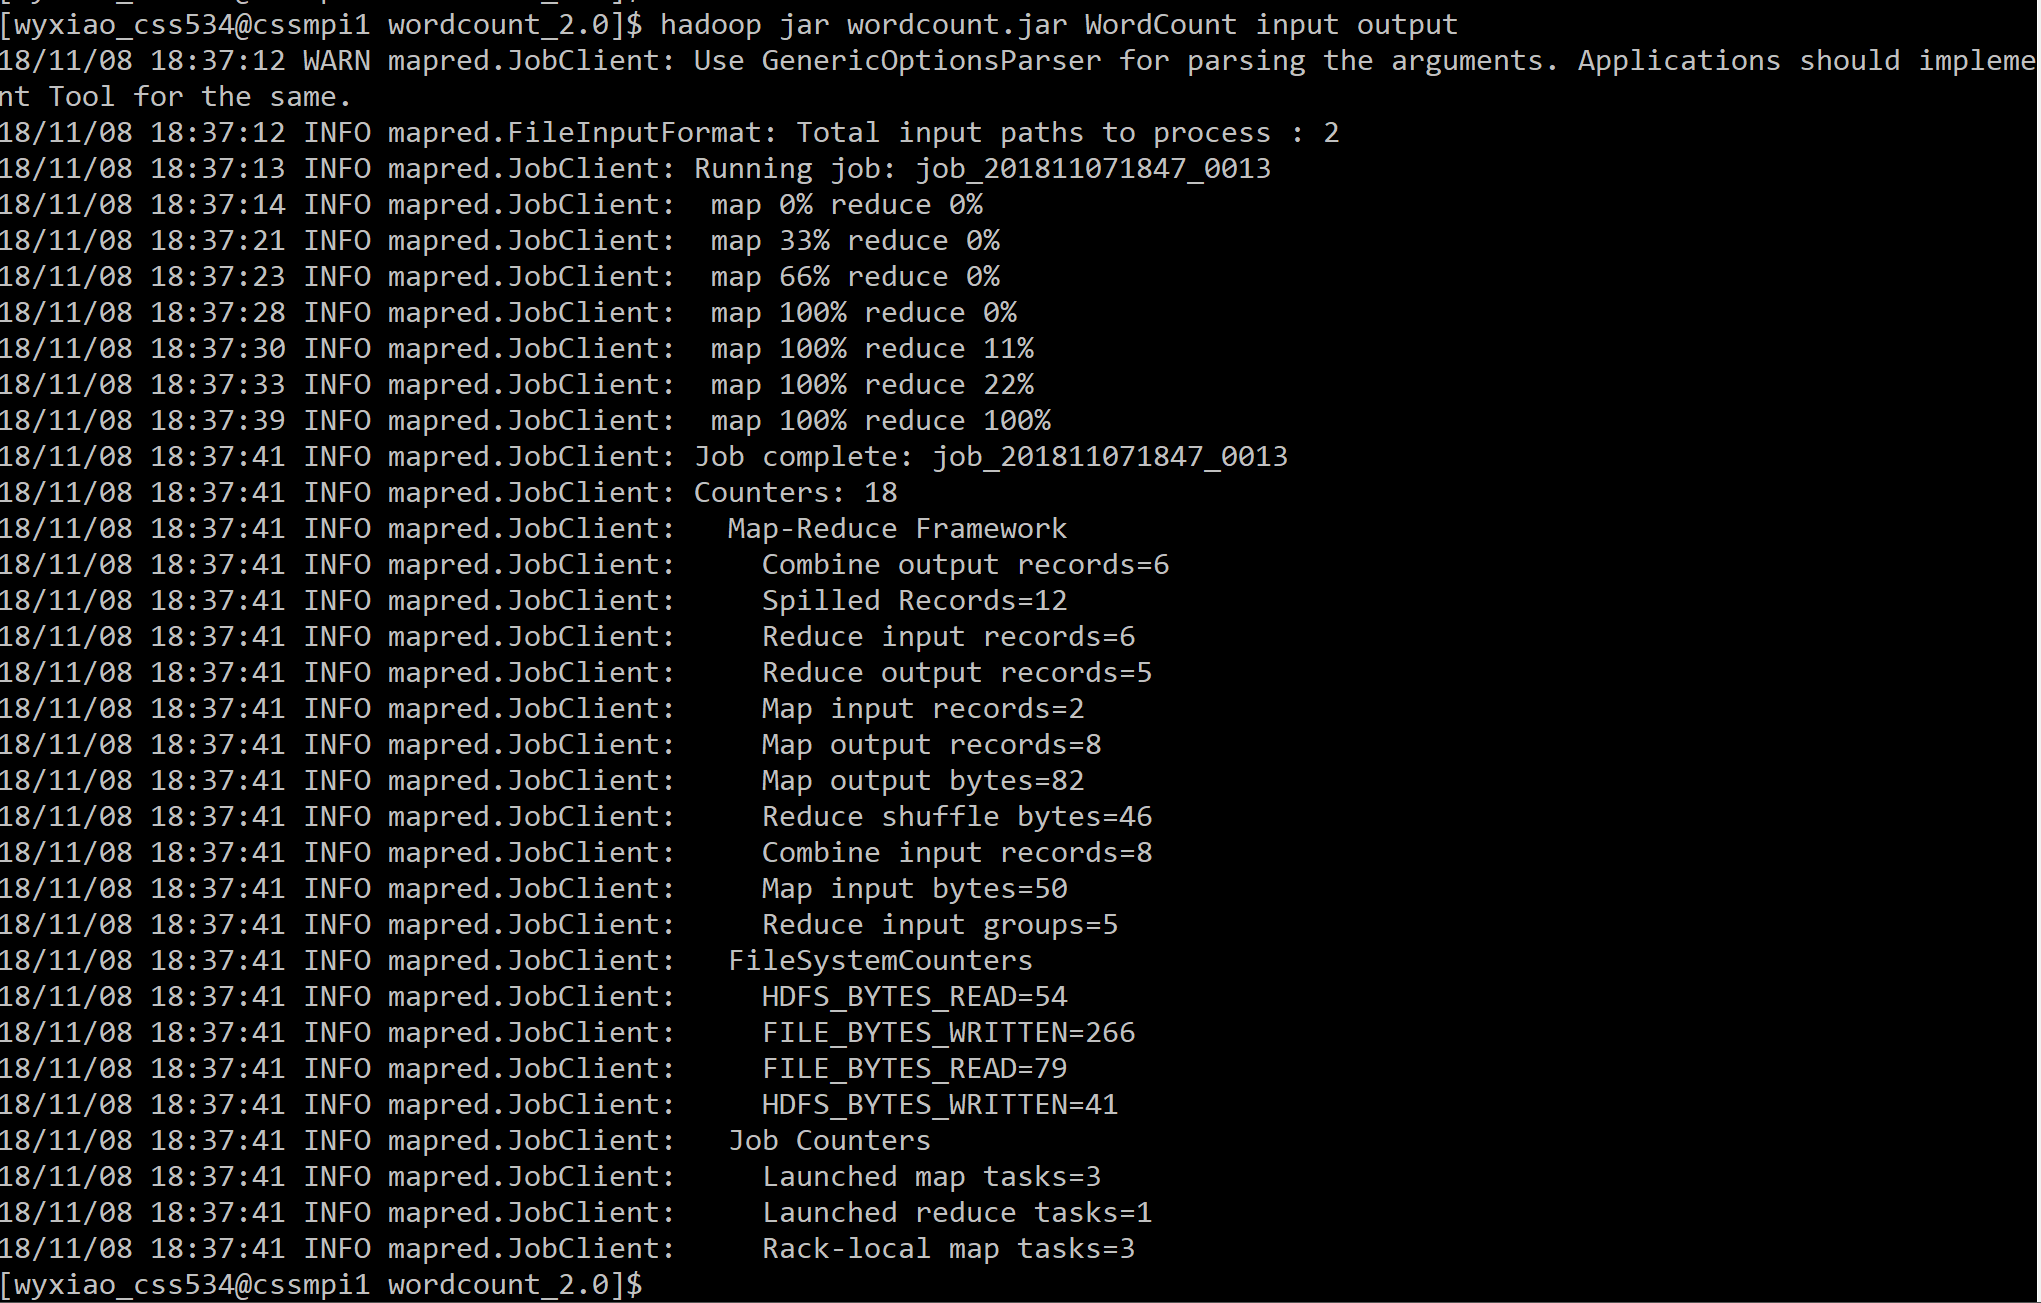
\includegraphics[width=0.7\textwidth]{lab3out0}
		\caption{MapReduce execution}
	\end{figure}
	
	\begin{figure}[h]
		\centering
		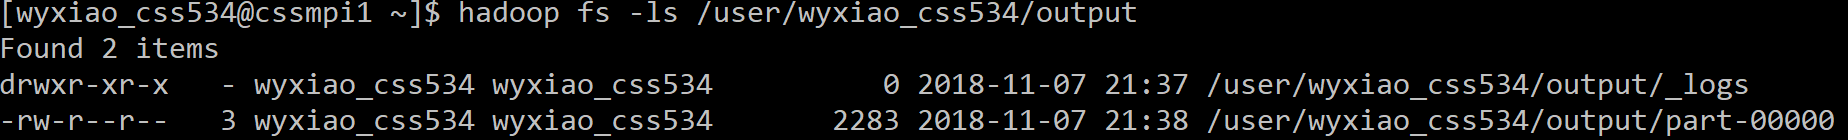
\includegraphics[width=0.7\textwidth]{lab3out1}
		\caption{/user/yourAccount/output}
	\end{figure}
	
	\begin{figure}[h]
		\centering
		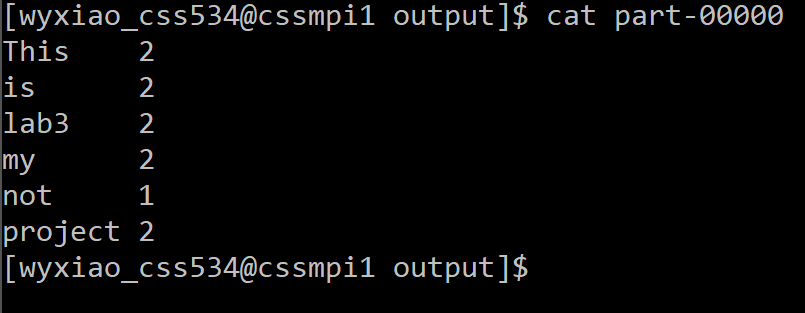
\includegraphics[width=0.7\textwidth]{lab3out2}
		\caption{part-00000}
	\end{figure}

\end{document}


















